\definecolor{datapolicy}{RGB}{68, 1, 84}
\definecolor{optimpolicy}{RGB}{49, 104, 142}

\definecolor{poptdraw}{RGB}{38, 130, 142}
\colorlet{poptd}{black!30!poptdraw}
\colorlet{poptds}{white!70!poptdraw}

\definecolor{naivetdraw}{RGB}{72, 40, 120}
\colorlet{naivetd}{black!30!naivetdraw}
\colorlet{naivetds}{white!70!naivetdraw}


\newcommand{\datapolicyglyph}[0]{\textls[10]{$\sqcdot\hspace{-.2em}\sqcdot\hspace{-.2em}\sqcdot$}}
\newcommand{\optimpolicyglyph}[0]{\raisebox{2pt}{\rule{8pt}{1.2pt}}}


A key problem in offline Reinforcement Learning (RL) is the mismatch between the dataset and the distribution over states and actions visited by the learned policy, called the \emph{distribution shift}. This is typically addressed by constraining the learned policy to be close to the data generating policy, at the cost of performance of the learned policy. We propose Projected Off-Policy TD (POP-TD), a new critic update rule that resamples TD updates to allow the learned policy to be distant from the data policy without catastrophic divergence. We evaluate our algorithm on a collection of offline RL benchmarks and show how various offline RL algorithms, notably Conservative Q-Learning (CQL), can be augmented to mitigate distribution shift. We show that when CQL is augmented with POP-TD, we improve performance with random data policies and mixed-expert policies.

\emph{From ``Projected Off-Policy TD Learning to Stabilize Offline Reinforcement Learning'' by \citeauthor{manek2023poptd} (\citeyear{manek2023poptd})}

\clearpage


\section{Introduction}

Reinforcement Learning (RL) aims to learn policies that maximize rewards in Markov Decision Processes (MDPs) through interaction, generally using Temporal Difference (TD) methods. In contrast, offline RL focuses on learning optimal policies from a static dataset sampled from an unknown policy, possibly a policy designed for a different task. Thus, algorithms are expected to learn without the ability to interact with the environment.
This is useful in environments that are expensive to explore (such as running a Tokamak nuclear reactor \cite{degrave2022magnetic}), or high-dimensional environments with cheap access to expert or near-expert trajectories (such as video games). \citet{levine2020survey} present a comprehensive survey of the area.

Since in offline RL the data is gathered before training begins, there is a mismatch between the the state-distributions implied by the learned policy and the data.
When applying naive RL algorithms in this setting, they tend to bootstrap from regions with little or no data, causing runaway self-reinforcement.S
Offline RL algorithms like Conservative Q-Learning (CQL) \cite{kumar2020cql}, on the other hand, generally constrain the learned policy to remain within the support of the data. While this works well in practice, there still remains a large gap in performance between online and offline RL. One reason for this is an additional subtlety to distribution shift: because of the combination of off-policy RL and function approximation, it is possible for RL to diverge if the generating policy and the learned policy are sufficiently different.

\begin{figure}[t]
  \centering
  \begin{tikzpicture}
    \tikzset{
        table/.style={
                matrix of nodes,
                row sep=-\pgflinewidth,
                column sep=-\pgflinewidth,
                nodes={
                        rectangle,
                        draw=black,
                        align=center,
                        text width=2.5em,
                    },
                minimum height=2.5em,
                text depth=0.5ex,
                text height=2ex,
                nodes in empty cells,
            }
    }

    \matrix (m) [table,text width=6em]
    {
         &   &   & S \\
         & X &   & X \\
         &   &   &   \\
         &   & X & G \\
    };

    \draw [-to,color=datapolicy,line width=1.2pt,densely dotted]
    ([yshift=2pt,xshift=-4pt]m-1-4.center) -- ([yshift=2pt]m-1-1.center)
    ([yshift=2pt]m-1-1.center) -- (m-4-1.center)
    (m-4-1.center) -- (m-4-2.center)
    (m-4-2.center) -- ([yshift=-2pt]m-3-2.center)
    ([yshift=-2pt]m-3-2.center) -- ([yshift=-2pt,xshift=-3pt]m-3-4.center)
    ([yshift=-2pt,xshift=-3pt]m-3-4.center)[shorten >=4pt] -- ([xshift=-3pt]m-4-4.center);

    \draw [-to,color=optimpolicy,line width=1.2pt]
    ([yshift=-2pt,xshift=-4pt]m-1-4.center) -- ([yshift=-2pt]m-1-3.center)
    ([yshift=-2pt]m-1-3.center) -- ([yshift=2pt]m-3-3.center)
    ([yshift=2pt]m-3-3.center) -- ([yshift=2pt,xshift=3pt]m-3-4.center)
    ([yshift=2pt,xshift=3pt]m-3-4.center)[shorten >=4pt] -- ([xshift=3pt]m-4-4.center);

\end{tikzpicture}

  \caption{A simple grid environment illustrating distribution shift despite complete support. We wish to learn the optimal trajectory ({\color{optimpolicy} \optimpolicyglyph}) from a suboptimal data policy ({\color{datapolicy} \datapolicyglyph}) which is $\epsilon$-dithered to get sufficient coverage. When we apply Q-learning methods to this, training often diverges to arbitrarily poor values. This is a consequence of distribution shift. In this paper, we propose a technique to solve this divergence. }
  \label{fig:sopmap}
\end{figure}

We illustrate a simple case in Figure~\ref{fig:sopmap}, where a simple grid environment is designed to elicit the shortest trajectory from start (S) to goal (G). Agents can move one step in each cardinal direction, reaching the goal yields a unit reward, and the episode ends on reaching the goal or any marked cell (X). We generate a dataset by following a suboptimal data policy ({\color{datapolicy} \datapolicyglyph}) with sufficient dithering to guarantee that every state-action pair is represented. If we use a tabular Q-function, we can recover the optimal policy ({\color{optimpolicy} \optimpolicyglyph}) and obtain the true value function. When we use a linear Q-function, however, the error is much larger. We find that about half of random initializations lead to Q-functions that either diverge or converge to large error. This shows how even with full coverage of states and actions, distribution shift can be a significant source of error. We provide more details in Section~\ref{sec:expsimpleoffpolicy}.

\paragraph{Contributions}
In this paper, we introduce POP-TD, a novel method of mitigating the error from off-policy learning. We show theoretically that this method bounds the off-policy approximation error for TD-based RL methods. Finally, we illustrate empirically that POP-TD can improve performance on offline RL tasks.
%// TODO: Revisit after experiments are complete.

\section{Related Work}

\paragraph{Offline RL and distribution shift}
Offline RL deals with \emph{distribution shift}, the problem where the stationary distribution of the learned policy does not match the dataset distribution. This is a key source of instability \citep{chen2019information,levine2020survey}, and naive methods require exponentially many samples in the problem horizon to address this \citep{wang2020statistical}.

One approach to Offline RL is to constrain the action space to prevent straying from the data policy, as in Batch-Constrained deep Q-learning \citep{fujimoto2019off}. This idea is improved on by BEAR \citep{kumar2019stabilizing}, which allows learned policies to stray from the sampling policy under limited conditions. \citet{laroche2019safe} interpolate bootstraps from the learned policy or the sampled data, depending on the uncertainty of the value. Conservative Q-Learning (CQL) \citep{kumar2020cql} augments existing online actor-critic methods, regularizing out-of-distribution Q-value samples to prevent overestimation. We build on CQL in this paper.

Alternative approaches leverage a dynamics model that is also learned from the data: MOPO \citep{yu2020mopo} use ensembles to understand the epistemic uncertainty of the dynamics around states and penalize the value estimates of more uncertain states, \citet{tianhe2021combo} eschew explicit uncertainty modeling by penalizing out-of-support data generated by their dynamics models. By constraining the model to be no better than the original environment, MoREL \citep{kidambi2020morel} learns a surrogate MDP that can be optimized with an online RL algorithm. More unusual methods devise entirely different RL algorithms to address this. In particular, Advantage-weighted Regression \citep{peng2019advantage} decomposes the problem into individual components that are learnt in a supervised manner.

\paragraph{Off-Policy Learning} Instability from learning off-policy has also been studied in the classic RL literature.
First described by \citet{tsitsiklis1996analysis}, the use of TD learning, function approximation, and off-policy sampling may cause severe instability or divergence. This is known as the \emph{deadly triad} \citep[p.~264]{sutton2020reinforcement} and even if many variants of TD still converge, the quality of the solution at convergence may be arbitrarily poor \citep{kolter2011fixed}.


There are three existing lines of work in the literature that attempt to resolve this: regularization, Emphatic reweighing, and TD Distribution Optimization (TD-DO).
The first attempts to regularize TD, typically with $\mathcal L_2$-norm weight regularization. Alternative regularization schemes are $\mathcal L_1$ \citep{mahadevan2014proximal}, convex \citep{yu2017convergence}, and bounds propagation \citep{kumar2020discor}. There are well-documented failure modes related to regularization \cite{manek2022pitfalls}.
The second line started with Emphatic-TD, in which \citet{sutton2016emphatic} note that it is possible to reweigh samples obtained off-policy so they appear to be on-policy. Such methods learn the follow-on trace using Monte-Carlo methods (in the original), TD \citep{jiang2021learning,zhang2020provably} or techniques similar to TD \citep{hasselt2021expected}. The third method, TD-DO, works by solving a small optimization problem on each TD update to reweigh samples to satisfy Kolter's Non-Expansion Criterion, which we introduce in the next section.

\paragraph{Importance Sampling}
Importance sampling (IS) is a common tool used to improve policy evaluation using off-policy data \citep{precup2000eligibility}.
The key idea is to re-weight samples from the data distribution to match the on-policy distribution.
However, because the variance of the re-weighting terms scale exponentially with the trajectory length, approximating the IS weights can be challenging in practice.
Several methods have been proposed to mitigate this challenge and improve performance of IS in practice \citep{hallak2017consistent, gelada2019off, nachum2019dualdice, nachum2019algaedice, liu2018breaking}, but conservative and behavior-regularized methods tend to outperform IS methods on offline RL benchmarks \citep{fu2020d4rl}.
While our method is also performing a re-weighting of the data distribution, POP-TD does not require learning the high-variance IS weighting terms.
We show in practice this yields better off-policy performance. 
% // TODO \todo{Have experiments that show this to be the case.}


\subsection{Kolter's Non-Expansion Criterion (KNEC)}
Thus far we have left open the notion of a ``safe'' distribution to resample TD updates to. The on-policy distribution must be safe, but we need to establish a criteria for acceptable off-policy distributions. \citeauthor{tsitsiklis1996analysis} lay the groundwork for this by analyzing the training of on-policy TD as a dynamical system and showing that once TD reaches its fixed point, subsequent TD updates form a non-expansive mapping around that fixed point (\citeyear[lemma 4]{tsitsiklis1996analysis}), and therefore prove that on-policy TD does not diverge. 

\citet{kolter2011fixed} extend this analysis to the off-policy case, deriving a linear matrix inequality (LMI) under which the TD updates are guaranteed to be non-expansive around the fixed point. This is Kolter's Non-Expansion Criterion (\citeyear{kolter2011fixed}):
\begin{align}
  \E_{s\sim \mu, s'\sim p(\cdot|s)} & \left[\begin{bmatrix}
                                                \phi(s)\phi(s)^\top  & \phi(s)\phi(s')^\top \\
                                                \phi(s')\phi(s)^\top & \phi(s)\phi(s)^\top
                                              \end{bmatrix}\right] \succcurlyeq 0 . \label{eqn:knec}
\end{align}
For convenience, we write this as:
\begin{align}
& \E_{s\sim q}  [F(s)] \succcurlyeq 0 \text{, where} \\
& F(s) = \E_{s'\sim p(s'|s)}  \left[\begin{bmatrix}
                                     \phi(s)\phi(s)^\top  & \phi(s)\phi(s')^\top \\
                                     \phi(s')\phi(s)^\top & \phi(s)\phi(s)^\top
                                   \end{bmatrix}\right] .
\end{align}
KNEC is an expectation over some state distribution $q$ and transition distribution $p(s,s') = p(s'|s) \mu(s)$. Because it is an LMI, the satisfying state distributions $q$ form a convex subset. More details of this derivation are in Appendix~\ref{sec:knecfull}.

%%%%%%%%%%%%%%%%%%%%%%%%%%%%%%%%%%%%%%%%%%%%%%%%%%%%%%%%%%%%

\section{Problem Setting and Notation }

Consider the $n$-state Markov chain $(\mathcal S, P, R, \gamma)$, with state space $\mathcal S$, transition function $P : \mathcal{S} \times \mathcal{S} \to \mathbb{R}_+$, reward function $R : \mathcal S \to \mathbb R$, and discount factor $\gamma \in [0, 1]$. 
% $P \in \mathbb R^{n\times n}$ is the transition matrix, with $P_{ij}$ encoding the probability of moving from state $i$ to $j$.
Because the state-space is finite, it can be indexed as $\mathcal{S} = \{1, \ldots, n\}$.
This allows us to use matrix rather than operator notation.
The expected $\gamma$-discounted future reward of being in each state $V(s) \coloneqq \E \left[\left.\sum_{t=0}^\infty \gamma^t R(s_t) \right| s_0 = s \right]$ is called the value function.
The value function is consistent with Bellman's equation (in matrix form):
\begin{align}
  V = R + \gamma P V .
\end{align}
In the linear setting, we approximate the value function as $V(s) \approx w^\top \phi(s)$, where $\phi : \mathcal S \to \mathbb R^{k}$ is a fixed basis function and we estimate parameters $w \in \mathbb R^k$. In matrix notation, we write this as $V \approx \Phi w$.

In this work, we are interested in the offline learning setting, where the sampling distribution $\mu$ differs from the stationary distribution $\nu$.
In this setting, the TD solution is:
\begin{align}
  \Phi w & = \Pi_{\mu} (R + \gamma P \Phi w) ,
\end{align}
where $\Pi_\mu = \Phi(\Phi^\top D_{\mu} \Phi)^{-1}\Phi^\top D_{\mu}$ is the projection onto the column space of $\Phi$ weighted by the data distribution $\mu$ through the matrix $D_{\mu} = \diag(\mu)$. This projection may be arbitrarily far from the true solution, and so the error may be correspondingly large. The literature bounds the error as:
\begin{theorem}
The error at the TD fixed point is $\|\Phi w - V \|_{D_\mu}$. Lemma 6 from \cite{tsitsiklis1996analysis} bounds this in terms of error projecting $V$ onto the column space of $\Phi$:
\begin{align}
    \|\Phi w - V \|_{D_\mu} & \leq \frac{1}{1-\gamma} ~ \| \Pi_{\mu} V - V \|_{D_\mu} 
\end{align} \label{thm:boundTDError}
\end{theorem}

%%%%%%%%%%%%%%%%%%%%%%%%%%%%%%%%%%%%%%%%%%%%%%%%%%%%%%%%%%%%

\section{Projected Off-Policy TD (POP-TD) }

We propose an alternative approach to stabilizing off-policy training, based on Kolter's Non-Expansion Criterion \citep{kolter2011fixed}. POP-TD identifies a convex set of ``safe'' distributions that satisfy KNEC and reweighs TD updates to come from that set. In contrast to TD-DO, POP-TD uses solves a different optimization problem using a two-timescales update with fixed cost per iteration, allowing it to scale to real-world problems. A more thorough derivation is in \cref{app:derivation}.

We begin by deriving the projected off-policy update for Markov Chains, without a separate policy function. We will extend this derivation to support actions and Markov Decision Processes (MDPs) in Section~\ref{sec:popq}. Our algorithm resamples TD updates so they come from some distribution $q$ for which KNEC holds. Given input data $(x_1, x_2, \ldots)$, this is the same as finding a set of weights $q_1, q_2, \ldots$ such that
\begin{align}
  \sum_i q_i & \cdot F(x_i) \succcurlyeq 0
\end{align}
% We also need to constrain our choice of distribution $q$ to ensure the quality of the solution.

\begin{comment}
\citet{kolter2011fixed} achieve this by selecting $q$ that solves this optimization problem
\begin{align}
  \underset{q}{\text{minimize}}~\text{KL}(\mu||q) & \qquad \text{s.t. } ~ E_{s\sim q}[F(s)] \succcurlyeq 0 \label{eqn:kolter2011objective}
\end{align}
explicitly optimizing over the distributons using a primal-dual formulation that exploits the structure of the problem. The resultant algorithm, TD-DO, performs a first-order optimization method on a dual objective using quasi-Newton methods alongside every TD step.
\end{comment}

% A deceptively simple theoretical insight opens up a new algorithmic possibility.
% Instead of the M-projection objective in \cref{eqn:kolter2011objective}, we optimize the dual I-projection instead:
To constrain the effective distribution to be close to the data distribution, we choose to set it to the closest stable I-projection of $q$ on $\mu$. (This is different from TD-DO \citep{kolter2011fixed}, as explained in Appendix~\ref{sec:improj}.)
\begin{align}
  \underset{q}{\text{minimize}}~\text{KL}(q\,\|\,\mu) & \qquad \text{s.t. } ~ \E_{s\sim q}[F(s)] \succcurlyeq 0 \label{eqn:ouroptobj}
\end{align}
% By changing the objective, we are able to integrate its solution into the basic TD algorithm and solve these concurrently. This avoids the first-order optimization in each update step, greatly reducing the time-complexity of the resultant algorithm. By switching to an I-projection, we may even improve the quality of the closest distribution $q$.

The dual of \cref{eqn:ouroptobj} can simplified (as detailed in Appendix~\ref{sec:distriboptim}):
\begin{align}
  \underset{Z \succcurlyeq 0}{\text{minimize}}~\E_{s \sim \mu} [\exp(\mathrm{tr} Z^\top F(s))] ,\label{eqn:ouroptobjdual}
\end{align}
where $Z \in \R^{2k \times 2k}$ is a Lagrange multiplier and we can obtain the optimal weights $q(s) \propto \mu(s) \exp(\mathrm{tr} Z^\top F(s))$. While this yields the optimal per-state weights, it is an impractically large optimization to solve. In the following we assume (and later verify) that $Z$ is low-rank and can be written as
\begin{align}
  Z & = \begin{bmatrix}
          Z_0 & - Z_0 \\ -Z_0 & Z_0
        \end{bmatrix} ,
  \intertext{which we approximate as rank-one with parameters $y\in \mathbb{R}^{k}$ following \citet{burer2003nonlinear}}
  Z & = \begin{bmatrix} y \\ -y \end{bmatrix}
  \begin{bmatrix} y \\ -y \end{bmatrix}^\top .
\end{align}
Substituting this into \cref{eqn:ouroptobjdual}, this objective simplifies to the unconstrained optimization problem
\begin{align}
  \underset{y}{\text{minimize}}~\E_{s\sim\mu} [\exp(y^\top A(s) y)]\text{, where}
  \label{eqn:outoptobjunconstr}
  \\ A(s) = \E_{s'\sim p(s'|s)} [\phi(s)(\phi(s) - \phi(s'))^\top]. \label{eqn:amatrix}
\end{align}
To solve this problem alongside TD learning we adopt a two-timescales method that separately estimates $y$ and $(y^\top A(s) y)$. To minimize the memory overhead, we directly represent $y \in \mathbb R^{k}$ (which is the same size as the learned weights), but approximate $g_\theta(s) = (y^\top A(s) y)$ using a separate function approximator with parameter $\theta$.

Differentiating the objective in \cref{eqn:outoptobjunconstr} with respect to $y$, we obtain:
\begin{align}
   & \nabla_y \mathbf{E}_\mu \left [ \exp (y^T A(s) y) \right ]
  \\ & =
  \E_{s \sim \mu, s' \sim p(\cdot|s)} \left [ \exp(2 g_\theta(s)) \phi(s)(\phi(s) - \phi(s'))^T y \right ] \nonumber
\end{align}
With this we can determine the update rules for POP-TD. At each step, $t$, of the underlying TD algorithm, we drive each parameter towards the objective values:
% \begin{align}
%   g_\theta(s) & \to (\phi(s)^\top) y \cdot (\phi(s)^\top - \phi(s')^\top) y
%   \\ y           & \to \exp{g_\theta(s)} (\phi(s)^\top - \phi(s')^\top) y \cdot \phi(s)
%   \intertext{Alongside these two update rules, we augment the TD update to reweigh each sample:}
%   w           & = w - \alpha \exp(2 g_\theta(s)) (\phi(s)^\top w - r - \phi(s')^\top w) \cdot \phi(s)
% \end{align}
\begin{align}
  g_{\text{target}, t}(s) &\gets \phi(s)^\top y \cdot (\phi(s) - \phi(s'))^\top y \\
  \theta_{t+1} &\gets \theta_t - \alpha_\theta \nabla_{\theta_t} (g_{\theta_t}(s) - g_{\text{target}, t}(s)) \\
  y_{t+1} &\gets y_t - \alpha_y \exp{g_\theta(s)} (\phi(s) - \phi(s'))^\top y \cdot \phi(s)
\end{align}
Alongside these two update rules, we augment the TD update to reweigh each sample by a factor of $\exp(2 g_\theta(s))$:
\begin{align}
  w & \gets w - \alpha \exp(2 g_\theta(s)) (\phi(s)^\top w - r - \phi(s')^\top w) \cdot \phi(s)
\end{align}
where $\alpha$ is a learning rate parameter.

\subsection{POP-Q-Learning}\label{sec:popq}

We now extend this from simple Markov chains to MDPs by incorporating actions into it. An MDP is a tuple, $(\mathcal{S}, \mathcal{A}, P, R, \gamma)$, with state space $\mathcal S$, transition function $P : \mathcal{S} \times \mathcal{A} \times \mathcal{S} \to \mathbb{R}_+$, reward function $R : \mathcal S \times \mathcal{A} \to \mathbb R$, and discount factor $\gamma \in [0, 1]$.
The goal in this setting is to find a probabilistic policy $\pi : \mathcal{S} \times \mathcal{A} \to \mathbb{R}_+$ that maximizes the future discounted reward:
\begin{equation}
    \pi^\star = \argmax_\pi \E_\pi \left [ \sum_{t=0}^\infty \gamma^t R(s_t, a_t) \right ]
\end{equation}
Many RL methods use variations of Q-learning \cite{kumar2020cql,watkins1992q,mnih2013playing,haarnoja2018soft}, which involves learning a state-action value function, or $Q$-function:
\begin{equation}
    Q^\pi(s, a) = \E_\pi \left[\left.\sum_{t=0}^\infty \gamma^t R(s_t, a_t) \right| s_0 = s, a_0 = a \right]
\end{equation}

By considering a fixed policy $\pi$, a combined state-space $\mathcal{X} = \mathcal{S} \times \mathcal{A}$, and a policy-conditioned transition function $\tilde{P}^\pi((s, a), (s', a')) = P(s, a, s') \pi(s', a')$, any MDP reduces to a Markov Chain.
Thus, as long as KNEC is satisfied in this modified state-space, we can bound the approximation error of the Q-function.
See \cref{app:pop-q-derivation} for a detailed derivation.

Now, the POP-TD update rules for this modified state-space become
\begin{align}
  g_\theta(s, a) \gets (\phi(s, a)^\top) y \cdot (\phi(s,a )^\top - \phi(s', \pi(s'))^\top) y \\
  y \gets \exp{g_\theta(s,a)} (\phi(s,a)^\top - \phi(s', \pi(s'))^\top) y \cdot \phi(s, a)
\end{align}
with
\begin{align}
  w \gets w - (\phi(s, a)^\top) y \cdot (\phi(s,a )^\top - \phi(s', \pi(s'))^\top) y \\
  y \gets \exp{g_\theta(s,a)} (\phi(s,a)^\top - \phi(s', \pi(s'))^\top) y \cdot \phi(s, a)
\end{align}


\section{Experiments and Discussion}

We first apply POP-TD to a well-understood example so that we can directly illustrate the how it resamples TD updates to a ``safe'' distribution. We use the simple three-state task from \cite{manek2022pitfalls}, including their specified transition function, value function, and basis. Since this is a policy evaluation task, there is no policy to be separately learned. Full details in this task are in \cref{app:threestate}.

For illustration purposes, we select the family of distributions $\pi = (\sfrac h 2, \sfrac h 2, 1- h)$ parameterized by $h \in [0, 1]$.
This characterizes the possible distributions of data that we will present to POP-TD and naive TD in this experiment. The on-policy distribution corresponds to $h_o\approx 0.51$, and divides the family of distributions into a left subset ($h \leq h_o$) where KNEC holds and a right subset ($h_o > 0.5$) where KNEC does not. This is immediately apparent in \cref{fig:threestate}, where we plot the error at convergence from running naive- and POP-TD above, and the effective distribution of TD updates after reweighing below.
In the left subset, where KNEC holds, POP-TD does not resample TD updates at all. Therefore, the error of POP-TD tracks naive TD (top), and the effective distribution of TD updates in POP-TD and naive TD are the same as the data distribution (bottom).

In the right subset, we observe that naive TD converges to poor solutions with large error while POP-TD is able to learn with low error.
Directly computing the effective distribution, we see that naive TD adheres to the data distribution but POP-TD resamples the TD updates.
Looking at the behavior of POP-TD in the right subset, we see that POP-TD resamples updates to the on-policy distribution $p_o$ in $p\in[p_o,0.9]$, corresponding to the horizontal segment. This allows the learned Q-function to have very low error in that domain. As the data distribution becomes more extreme ($p\in [0.9, 1)$), POP-TD is not quite able to learn the resampling ratio, and so the effective distribution shifts away from $p_o$. This leads to a corresponding slight increase in error at extreme ratios. From this we observe that POP-TD requires full support of the sampling distribution, similar to many offline RL algorithms \cite{kumar2020cql,shi2022pessimistic}.

This simple experiment cleanly illustrates how POP-TD resamples TD updates to come from a ``safe'' distribution, and how that can greatly reduce the error in a policy evaluation task.

\label{sec:threestateexp}
\begin{figure}[t]
  \centering
  \begin{tikzpicture}
    \begin{groupplot}[
        group style={
                % set how the plots should be organized
                group size=1 by 2,
                % only show ticklabels and axis labels on the bottom
                x descriptions at=edge bottom,
                % set the `vertical sep' to zero
                vertical sep=0pt,
            },
        width=1.\columnwidth,
        height=.6\columnwidth,
        xmin=0, xmax=1,
        xlabel={Distrib. param. $h$, where $\pi = [\sfrac h 2, \sfrac h 2, 1-h]$},
        ]

        \nextgroupplot[
            ylabel={$\log_{10}$ Error},
            ymode=log,
            ymin=0.00001, ymax=1000,
            yticklabels={-5,-1,3}
        ]

        \addplot [color=poptd] table [x index=0,y index=1] {poptd/threestate/export_threestate.dat};
        \node at (axis cs:.75,0.0001) [anchor=south west,color=poptd] {POP-TD};

        \addplot [color=naivetd,dashed] table [x index=0,y index=2] {poptd/threestate/export_threestate.dat};
        \node at (axis cs:.75,1.) [anchor=north west,color=naivetd] {Naive TD};
        % \addlegendentry{Naive TD}

        \node at (axis cs:.514,1000) [anchor=north east] {$F(s)\succcurlyeq 0$};
        \node at (axis cs:.514,1000) [anchor=north west] {$F(s)\not\succcurlyeq 0$};
        \draw[dotted,thick] (axis cs:0.514,0.0000001) -- (axis cs:0.514,1000000);

        \nextgroupplot[
            ylabel={effective distrib. $p$},
            ymin=0., ymax=1.,
            yticklabels={,0,.2,.4,.6,.8,}
        ]

        \addplot [color=poptd] table [x index=0,y index=3] {poptd/threestate/export_threestate.dat};
        \node at (axis cs:.75,.5) [anchor=north east,color=poptd] {POP-TD};

        \addplot [color=naivetd, domain=0:1,dashed] {x} ;
        \node at (axis cs:.75,.75) [anchor=south east,color=naivetd] {Naive TD};

        \draw[dotted,thick] (axis cs:0.514,0.) -- (axis cs:0.514,1);

    \end{groupplot}

\end{tikzpicture}

  \caption{The error in the learned value function by naive- and POP-TD, plotted against a varying sampling distribution. In the left half of the plot, KNEC holds, and so POP-TD tracks the error of naive TD closely. In the right half of the plot naive TD diverges, while POP-TD resamples the data to a ``safe'' distribution and does not diverge. }
  \label{fig:threestate}
\end{figure}



\subsection{POP-Q on GridWorld}

\label{sec:expsimpleoffpolicy}
\begin{figure}[t]
  \centering
  \begin{tikzpicture}
    \begin{axis}[
            width=1.\columnwidth,height=1.\columnwidth,
            xmin=-4, xmax=7,
            ymin=-4, ymax=7,
            xlabel=log Naive Error,
            ylabel=log POP-Q Error,
            ylabel style={
                    yshift = {-1.5*height("0") },
                },
            ymajorgrids=true,
            yminorgrids=true,
            minor tick num=1,
            minor y grid style={line width=.2pt,draw=gray!20},
            major y grid style={line width=.2pt,draw=gray!50},
        ]

        \addplot[black,domain=-4:7] {x};
        \addplot[only marks,mark=+,mark options={viridis09}] table[x=log_error_naive, y=log_error_pop] {poptd/simpleoffpolicy/qval_err.dat};


        \node at (axis cs:-1.22,7) [anchor=north west,color=black!50!viridis02] {Mean On-Policy Error};
        %\draw[black!50!viridis02,dotted,thick] (axis cs:7,-1.22) -- (axis cs:-1.22,-1.22) -- (axis cs:-1.22,7);
        \draw[black!50!viridis02,dotted,thick] (axis cs:7,-1.22) -- (axis cs:-5,-1.22);
        \draw[black!50!viridis02,dotted,thick] (axis cs:-1.22,-5) -- (axis cs:-1.22,7);
    \end{axis}

\end{tikzpicture}

  % \vspace{-1.75em}
  \caption{Q-function errors for naive and POP Q-Learning on \cref{fig:sopmap}, over 50 randomly sampled bases. Points below the line correspond to bases where POP-Q has lower error. POP-Q substantially reduces error at convergence in about half the sampled bases. }
  \label{fig:soperr}
\end{figure}

% We motivated this paper with the simple grid environment in \cref{fig:sopmap}.
In this experiment, we consider the the simple grid environment from \cref{fig:sopmap}.
Our training data is sampled following the suboptimal data policy ({\color{datapolicy} \datapolicyglyph}), adding uniform random dithering to guarantee that every state-action pair is represented.
Our goal is to approximate the true Q-function, eventually recovering the optimal policy ({\color{optimpolicy} \optimpolicyglyph}).
We represent the Q-function as a linear function with a fixed random basis, training it to convergence using naive Q-learning and POP-Q separately. (For POP-Q, we also randomly initialize a tabular $y$ and $g$ separately.) We also compute the ground-truth Q-function using tabular Q-learning, which must converge to the global optimum \cite{watkins1992q}.

We plot the error at convergence over 50 different random initializations in \cref{fig:soperr}, where the horizontal position of the point indicates the error when Naive TD is used, and the vertical position indicated the error with POP-TD. About half of the points are below the diagonal line, indicating that POP-Q has lower error in those cases. For comparison, we annotate the mean error if similarly-initialized Q-functions were trained following the optimal policy (\emph{On-Policy}), which represents the best-case error in expectation.

The distribution of errors in naive Q-learning spans many orders of magnitude. This is expected because we have deliberately engineered the task to be unstable. The stability of TD in each case depends on the basis (see \cref{eqn:koldercondstate}), which is randomly sampled. By comparing the performance between POP-TD and naive TD on the with the same basis, we can show that POP-TD is able to mitigate instability on bases where naive TD is unstable.

POP-Q attempts to resample updates to find a distribution where KNEC holds. We can indirectly observe this tendency by finding the smallest eigenvalue of the A-matrix (from \cref{eqn:amatrix}), and comparing it before and after reweighing. In 90\% of the cases, the smallest eigenvalue increases after reweighing, suggesting that POP-Q is successfully resampling the data to a distribution closer to one where KNEC holds.

% // TODO \todo{Gaurav: Add results for non-random policy.}
\begin{table}[t]
  \centering
  \begin{tabular}{lr@{\,}c@{\,}lr@{\,}c@{\,}l}\hline\hline
\texttt{*-random-v2} & \multicolumn{3}{c}{POP-CQL} & \multicolumn{3}{c}{CQL}
\\\hline
  	\texttt{hopper}      & 0.064 & $\pm$ & 0.007 & 0.064 & $\pm$ & 0.007
\\	\texttt{halfcheetah} & 0.306 & $\pm$ & 0.028 & 0.288 & $\pm$ & 0.098
\\	\texttt{walker2d}    & 0.105 & $\pm$ & 0.060 & 0.057 & $\pm$ & 0.002
\\	\texttt{ant}         & 0.191 & $\pm$ & 0.097 & 0.353 & $\pm$ & 0.096
\\ \hline\hline
  \end{tabular}
  \caption{Performance of POP-CQL vs vanilla CQL on a range of datasets, expressed as the normalized score following the D4RL formula. 0 corresponds to the score that a random policy would achieve, and 1 corresponds to an SAC agent trained interactively. D4RL offers improvements on some locomotion environments when trained on data following a random policy. }
  \label{tab:resultsd4rl}
\end{table}


% POP-Q resamples data to the closest distribution satisfying KNEC, which is not necessarily the on-policy distribution so the errors in the learned models are generally not as low as sampling on-policy. We also note a few cases in which the error increases; this happens when TD-updates are non-expansive, but cannot be cerified as such by KNEC. As KNEC describes a convex subset of non-expansive distributions it may exclude ``safe'' distributions, which causes needless resampling.

\subsection{D4RL Random Datasets}

\begin{figure}[t]
  \centering
  \begin{tikzpicture}
    \begin{axis}[
            width=1.\columnwidth,height=.6\columnwidth,
            xmin=0, xmax=1600,
            ymin=0.19, ymax=0.33,
            ylabel={Normalized Reward},
            ytick={0.2,0.24,0.28,0.32},
            yticklabels={20,24,28,32},
            xtick={0, 400, 800, 1200, 1600},
            legend style={legend cell align=left,at={(0.5,-0.15)},anchor=north,legend columns=3},
        ]

        \addplot [name path=poptdU,color=poptd!20] table [x=step,y expr=(\thisrow{ci_upper}-\thisrow{average_return})/2.828 + \thisrow{average_return},forget plot] {poptd/d4rl/returns_halfcheetah-random-v2_popcql.tsv};
        \addplot [name path=poptdL,color=poptd!20] table [x=step,y expr=(\thisrow{ci_lower}-\thisrow{average_return})/2.828 + \thisrow{average_return},forget plot] {poptd/d4rl/returns_halfcheetah-random-v2_popcql.tsv};
        \addplot[color=poptd!20,forget plot] fill between[of=poptdU and poptdL];

        \addplot [name path=naivetdU,color=naivetd!20,forget plot] table [x=step,y expr=(\thisrow{ci_upper}-\thisrow{average_return})/2.828 + \thisrow{average_return}] {poptd/d4rl/returns_halfcheetah-random-v2_cql.tsv};
        \addplot [name path=naivetdL,color=naivetd!20,forget plot] table [x=step,y expr=(\thisrow{ci_lower}-\thisrow{average_return})/2.828 + \thisrow{average_return}] {poptd/d4rl/returns_halfcheetah-random-v2_cql.tsv};
        \addplot[color=naivetd!20,forget plot] fill between[of=naivetdU and naivetdL];

        \addplot [name path=dualdiceU,color=dualdice!20,forget plot] table [x=step,y expr=(\thisrow{ci_upper}-\thisrow{average_return})/2.828 + \thisrow{average_return}] {poptd/d4rl/returns_halfcheetah-random-v2_dualdicecql.tsv};
        \addplot [name path=dualdiceL,color=dualdice!20,forget plot] table [x=step,y expr=(\thisrow{ci_lower}-\thisrow{average_return})/2.828 + \thisrow{average_return}] {poptd/d4rl/returns_halfcheetah-random-v2_dualdicecql.tsv};
        \addplot[color=dualdice!20,forget plot] fill between[of=dualdiceU and dualdiceL];


        \addplot [color=black!30!dualdice, forget plot] table [x=step,y=average_return] {poptd/d4rl/returns_halfcheetah-random-v2_dualdicecql.tsv};
        \addlegendimage{dualdice,line width=3pt}
        % \addlegendimage{dualdice}
        \addlegendentry{DualDICE + CQL};
        \addplot [color=black!30!poptd,forget plot] table [x=step,y=average_return] {poptd/d4rl/returns_halfcheetah-random-v2_popcql.tsv};
        \addlegendimage{poptd,line width=3pt}

        \addlegendentry{POP-CQL};
        \addplot [color=black!30!naivetd,forget plot] table [x=step,y=average_return] {poptd/d4rl/returns_halfcheetah-random-v2_cql.tsv};
        \addlegendimage{naivetd,line width=3pt}
        \addlegendentry{CQL};

    \end{axis}
\end{tikzpicture}

  \caption{
    POP-Q learning performs slightly but significantly better than naive Q learning on the D4RL dataset \texttt{halfcheetah-random-v2}. The plot is smoothed, and shaded sections represent the standard error over 18 seeds. POP-Q can help us deal with datasets generated by vastly different policies.}
  % TODO: Report normalized reward instead.
  \label{fig:d4rl}
\end{figure}
%// TODO \todo{Mel: Also, we should keep the number of iterations consistent between experiments. Otherwise it looks suspicious. Gaurav: I'll rerun these shortly.}


One application of POP techniques is to improve learning from sub-optimal offline data. To illustrate this, we augment Conservative Q-Learning (CQL) by \citet{kumar2020cql} with our projected off-policy technique for better offline RL. The resultant algorithm, called POP-CQL, parameterizes the Q-function and $g_\theta(s, a)$ as separate neural networks. We still learn a linear $y$, treating the output of the penultimate layer of the Q-function as the basis. The use of CQL is important because it ensures the learned policy remains within the support of the data, which our toy experiments suggest is necessary.

We run CQL and POP-CQL on the \texttt{halfcheetah-random-v2} dataset from D4RL \citep{fu2020d4rl}, which consists of $10^6$ samples from the \texttt{HalfCheetah} OpenAI Gym \citep{openaigym} environment following random actions. Running over twenty random seeds, we discard the two lowest-performing seeds from CQL and POP-CQL (in which training fails and we obtain negative reward.) We plot the mean performance over the remaining seeds in \cref{fig:d4rl}, along with the $10^\text{th}$ and $90^\text{th}$ percentile confidence bounds. We see that POP-CQL performs slightly -- but significantly -- better than vanilla CQL!

This is one example of how POP-Q can help us deal with datasets where the data policy is very different from the optimal policy. We include further experimental outcomes in Table~\ref{tab:resultsd4rl}
Running a similar test on other \texttt{HalfCheetah-v2} D4RL datasets generated by expert actions, POP-CQL no longer provides any advantage over CQL. This is expected, since the data distribution is closer to the optimal policy in this case. To illustrate a case where POP-Q is helpful despite a non-random data policy, we consider mixed-policy datasets as well.

\subsection{Mixed-Policy Datasets}

Finally, our POP technique allows us to learn when multiple policies are mixed, even when part of the dataset comes from a potentially adversarial policy. This is especially relevant if we wish to learn from expert-produced data that comes from different experts, or if the dataset may include samples from adversaries.

To illustrate this, we generate a custom dataset in the style of D4RL. Using the \texttt{HalfCheetah} environment from BRAX \citep{brax2021github}, we combine $250,000$ samples generated by an adversarial policy that runs backwards (achieving $-3000$ score per trajectory) with $50,000$ samples generated by an expert policy (achieving about $7000$ per trajectory). We train both CQL and POP-CQL on the resultant dataset and plot the performance in \cref{fig:fwdback}, which shows that POP-Q learning performs better on average than naive Q learning in this situation. Due to the large amount of adversarial data, training is volatile.

\begin{figure}[t]
  \centering
  # TODO: Do not use this without changing the data. 
\begin{tikzpicture}
    \begin{axis}[
            width=\columnwidth,height=.6\columnwidth,
            xmin=1, xmax=1000,
            ymin=0.0, ymax=5.5,
            ylabel=Reward ($\times10^3$),
        ]

        \addplot [name path=poptdU,color=poptd!20] table [x=I,y expr=(\thisrow{POPS}+\thisrow{POPCIS})/1000] {poptd/fwdback/fwdback.dat};
        \addplot [name path=poptdL,color=poptd!20] table [x=I,y expr=(\thisrow{POPS}-\thisrow{POPCIS})/1000] {poptd/fwdback/fwdback.dat};
        \addplot[poptd!20] fill between[of=poptdU and poptdL];
        %\addplot[pattern color=poptd!20,pattern=north west lines,] fill between[of=poptdU and poptdL];

        \addplot [name path=naivetdU,color=naivetd!20] table [x=I,y expr=(\thisrow{NOPOPS}+\thisrow{NOPOPCIS})/1000] {poptd/fwdback/fwdback.dat};
        \addplot [name path=naivetdL,color=naivetd!20] table [x=I,y expr=(\thisrow{NOPOPS}-\thisrow{NOPOPCIS})/1000] {poptd/fwdback/fwdback.dat};
        \addplot[pattern color=naivetd!20,pattern=north east lines,] fill between[of=naivetdU and naivetdL];

        \addplot [color=poptd] table [x=I,y expr=\thisrow{POPS}/1000] {poptd/fwdback/fwdback.dat};
        \addplot [color=naivetd] table [x=I,y expr=\thisrow{NOPOPS}/1000] {poptd/fwdback/fwdback.dat};


        \node at (axis cs:1000,4.500) [anchor=south east] {{\color{poptd} POP-Q}};
        \node at (axis cs:1000,2.500) [anchor=north east] {{\color{naivetd} Naive Q}};

    \end{axis}
\end{tikzpicture}

  \caption{
    On custom mixed-policy dataset, POP-Q learning performs better than naive Q learning. The plot is smoothed, and shaded sections represent the 10\% and 90\% confidence bound over 10 seeds. POP-Q can help us deal with datasets generated by vastly different policies.
  }
  % No normalized reward is available for our dataset.
  \label{fig:fwdback}
\end{figure}

\section{Conclusion}
In this paper, we introduce a method for decreasing the approximation error off-policy for both state value functions, POP-TD, and state-action value functions, POP-Q.
We prove that, under mild assumptions, our method guarantees that the off-policy approximation error for both state and state-action value functions is bounded.
In our small-scale experiments we show that this method significantly decreases the approximation error for certain sampling functions, while never significantly increasing the error.
We also show that this method can be combined with Conservative Q-Learning to improve performance on ....


\section{POP-TD Details}
\label{app:derivation}

This is a more detailed derivation of the theory behind this project, starting from Kolter's non-expansion condition \citep{kolter2011fixed} and ending with the production of the update rules.

\subsection{I- and M-projections} \label{sec:improj}
The Kullback-Leibler divergence is an \emph{asymmetric} measure, and so it is usually the case that $\min_q~\text{KL}(q||\mu) \neq \min_q~\text{KL}(\mu||q)$. The former (``from $\mu$ to $q$'') is an information (or I-)projection, which tends to under-estimate the support of $q$ potentially excluding possible sampling distributions to reweigh to. The latter (``from $q$ to $\mu$'') is a moment (or M-)projection, which tends to over-estimate the support of $q$ and avoid zero solutions. In our solution, we are proposing using an I-projection instead of the M-projection used by \citet{kolter2011fixed}.

\subsection{Kolter's non-expansion condition}
\label{sec:knecfull}
Let $D = \diag(\pi)$. Error bounds from on-policy TD follow the property that the $D-$norm of any vector $x \in \mathbb R^n$ is non-expansive through the transition matrix. That is: $\|Px\|_D \leq \|x\|_D$. \citet{kolter2011fixed} observes that we relax this to potentially off-policy distributions $D$. Theorem 2 of \cite{kolter2011fixed} bounds the error of the TD update as:
\begin{align}
  \|\Phi w - V\|_D    & \leq \frac{1 + \gamma \kappa(D^{-\sfrac{1}{2}}D^{\sfrac{1}{2}})}{1 - \gamma} \|\Pi_D V - V\|_D
  \intertext{From this bound, he derives \emph{Kolter's non-expansion condition}:}
  \|\Pi_D P\Phi w\|_D & \leq \|\Phi w\|_D \qquad (\forall w \in \mathbb R^n) \label{eqn:kolterthm2bound}
  \intertext{This holds if and only if the matrix $F_D$ is positive semi-definite}
  F_D                      & \equiv \begin{bmatrix}
                                      \Phi^\top D \Phi        & \Phi^\top D P \Phi \\
                                      \Phi^\top P^\top D \Phi & \Phi^\top D \Phi
                                    \end{bmatrix} \succcurlyeq 0
\end{align}
This constraint describes a convex subset of $D$. As a $2k\times 2k$ matrix (where $k$ is the number of features), $F$ is prohibitively large to enumerate for any real RL problem, and so our algorithm is designed to make use of this without ever constructing it directly. Further, we notice that the construction of $F_D$ depends on $P$, the transition matrix of the underlying Markov process, which complicates how we construct it from samples.

Later in the algorithm, we will need to compute the contribution of a single sample to the expectation of $F$. To do this, we define the function $F(s, s')$ as the contribution of a single state-transition pair towards the construction of $F_D$. That is:
\begin{align}
  F(s, s')       & = \begin{bmatrix}
                       \phi(s)\phi(s)^\top & \phi(s)\phi(s')^\top
                       \\  \phi(s')\phi(s)^\top & \phi(s)\phi(s)^\top
                     \end{bmatrix}
  \intertext{and its expectation:}
  F_{\diag(\mu)} & = \E_{s\sim \mu, s'\sim p(\cdot|s)} F(s, s')
  \intertext{For convenience, we define the shorthand $F(s)$, noting that it depends on the transition distribution $p(\cdot|s)$.}
  F(s)           & = \E_{s'\sim p(\cdot|s)} F(s, s')
\end{align}

Directly constructing $F(s)$ or $F(s, s')$ is impossible on all but the simplest examples -- it would take $\mathcal O(k^2n)$ or $\mathcal O(k^2n^2)$ memory to hold all the necessary data. Instead we exploit the structure inherent in the problem to make use of $F(s)$ without creating it.

\subsection{Optimizing the distribution} 
\label{sec:distriboptim}

In the previous section we have characterized a convex subset of off-policy distributions under which TD learning is guaranteed not to diverge. If we can discover any such distribution for a particular TD problem, we can reweigh our TD updates (from any distribution) so they appear consistent with this reweighing distribution. This is related to the main insight in Emphatic-TD \citep{sutton2016emphatic}, with the key innovation that we can take any non-expansive distribution \emph{not just the on-policy distribution}.

We can now write down the optimization problem that we wish to solve:
\begin{align}
  \underset{q}{\text{minimize}}~\text{KL}(q||\mu) & \qquad \text{s.t. } ~ E_{s\sim q}[F(s)] \succcurlyeq 0
\end{align}
We are searching for $q$, the closest distribution to the sampling distribution $\mu$ such that $F$ is PSD under $q$. Note that we could in principle minimize any notion of ``closest'' to find some satisfying distribution -- for example \citet{kolter2011fixed} explores the effects of minimizing $\text{KL}(\mu||q)$.

We construct the dual of this problem:
\begin{align}
  \underset{Z\succcurlyeq 0}{\text{maximize}}~ \underset{q}{\text{minimize}}~\text{KL}(q||\mu) - \tr Z^\top \E_{s\sim q}[F(s)]
\end{align}
Using the Lagrange multiplier $Z\in\mathbb R^{2k\times 2k}$, we solve the inner optimization problem:
\begin{align}
  \underset{q}{\text{minimize}} - H(q) - \E_{s\sim q}[\log \mu(s) + \tr Z^\top F(s)]
\end{align}
Writing down Lagrangian and solving for the optima, we obtain:
\begin{align}
  q^*(s) & \propto \mu(s)\exp( \tr Z^\top F(s))
\end{align}
(Subject to the constraint that $q^*(s)$ is normalized so it must sum to 1 over all $s$.)

Plugging this back into our dual formulation, we obtain the optimization problem:
\begin{align}
  \underset{Z\succcurlyeq 0}{\text{maximize}}   & -\log \E_{s\sim\mu} [ \exp(\tr Z^\top F(s)) ]
  \intertext{Which we can simplify to}
  \underset{Z\succcurlyeq 0}{\text{minimize}} ~ & \E_{s\sim\mu} [ \exp(\tr Z^\top F(s)) ]
\end{align}

As discussed earlier, $F(s)$ cannot be directly constructed; instead, we assume that $Z$ holds a specific structure and optimize the problem.


\subsection{Simplifying the optimization problem}

Our next goal is to transform this constrained optimization problem into an unconstrained problem over a low-rank version of $Z$, suitable for learning via SGD.

We assume (and later check!) that the solution for $Z$ is low-rank. Intuitively, this is because $\E_{s\sim\mu}[F(s)]$ is PSD when $\mu$ is close to $\pi$, and for most MDPs, sampling off-policy leads to only a small number of negative eigenvalues that need to be corrected by $Z$. \citet{kolter2011fixed} provides a technical explanation: by the KKT conditions, $Z$ will have rank complementary to $\E_{s\sim\mu}[F(s)]$, and the latter is expected to be full rank. It is worth noting that this ``almost-PSD'' assumption is common in the field. We later discuss how we verify that this assumption holds.

We make the strong assumption that $Z$ is rank one, and apply the Burer-Montiero approach \citep{burer2003nonlinear} to convert the constrained optimization problem over $Z$ into an unconstrained optimization over $y\in \mathbb R^{k}$:
\begin{align}
  Z^\star & = \begin{bmatrix} y \\ -y \end{bmatrix} \begin{bmatrix} y \\ -y\end{bmatrix}^T
\end{align}
Substituting this into the dual formulation, we get:
\begin{align}
  \underset{y}{\text{minimize}} & \;\; \mathbf{E}_{s\sim\mu} \left [ \exp\left (\tr  \begin{bmatrix} y \\ -y \end{bmatrix} \begin{bmatrix} y \\ -y\end{bmatrix}^T F(s) \right )  \right ]
\end{align}

We can leverage the structure of $F(s)$ to simplify the trace term:
\begin{align}
   & \tr  \begin{bmatrix} y \\ -y \end{bmatrix} \begin{bmatrix} y \\ -y \end{bmatrix}^T F(s)
  \\ & = \begin{bmatrix} y \\ -y \end{bmatrix}^T F(s) \begin{bmatrix} y \\ -y \end{bmatrix}
  \\ & =  \begin{bmatrix} y \\ -y \end{bmatrix}^T  \mathbf{E}_{s' \sim p(s'|s)}  \left[ \begin{array}{cc} \phi(s)\phi(s)^T & \phi(s)\phi(s')^T \\ \phi(s')\phi(s)^T & \phi(s)\phi(s)^T \end{array} \right]
  \begin{bmatrix} y \\ -y \end{bmatrix}
  \\  & =  2 y^T \mathbf{E}_{s' \sim p(s'|s)} \left [\phi(s)(\phi(s)- \phi(s'))^T \right ] y
  \\  & =  2 y^T A(s) y
\end{align}

where $A(s) = \mathbf{E}_{s' \sim p(s'|s)} \left [\phi(s)(\phi(s)- \phi(s'))^T \right ]$

This allows us to rewrite the optimization problem as:
\begin{align}
  \underset{y}{\text{minimize}} & \;\; \mathbf{E}_{s\sim\mu} \left [ \exp\left(2 y^\top A(s) y \right)  \right ]
\end{align}

This has some great properties: in particular, we can optimize $y$ in an unconstrained manner (i.e. with SGD), and we need only use quantities that we already compute ($\phi(s), \phi(s')$). All this leads to the final step, the derivtion of the update rules:


\subsection{Update rules}

We can't directly optimize $y$ because that would require us to create $A(s)$. Instead, we use a two-timescales approach by estimating two (dependent) quantities separately and improving them at potentially different rates. By optimizing over the two quantities simultaneously, we hope to be able to discover the convergent value. This is generally possible with a little tuning.

We choose to optimize $y \in \mathbb R^k$ which is the same size as $w$, and the trace estimate $g(s) = y^\top A(s) y \in \mathbb R^n$. Instead of learning a tabular $g(s)$, we can approximate it as a linear function (or a neural network, for larger problems). This decision means the size of the per-update weights are still $\mathcal O(k)$ (limited by $w$ and $y$).

We find the derivative of the objective with respect to $g(s)$ and $y$ and use that to construct update rules for our algorithm.
\begin{align}
   & \nabla_y \mathbf{E}_\mu \left [ \exp (2 y^T A(s) y) \right ]
  \\ & =
  \mathbf{E}_{s \sim \mu(s)} \left [ \exp (2 y^T A(s) y) \; A(s) y \right ]
  \\  & = \mathbf{E}_{s \sim \mu(s), s' \sim p(s'|s)} \left [ \exp (2 y^T A(s) y) \; \phi(s)(\phi(s) - \phi(s))^T y \right ]
  \intertext{We substitute $g(s)$ into this to arrive at the final gradient derivation}
   & = \mathbf{E}_{s \sim \mu(s), s' \sim p(s'|s)} \left [ \exp(2 g(s)) \; \phi(s)(\phi(s) - \phi(s'))^T y \right ].
\end{align}

This corresponds to the update rules:
\begin{align}
  a      & \gets \phi(s)^\top y                                                    \\
  b      & \gets \phi(s')^\top y                                                   \\
  \theta & \gets \theta - \alpha_1 (g_\theta(s) - a(a-b))\nabla_\theta g_\theta(s) \\
  y      & \gets y - \alpha_2 \exp(2 g_\theta(s)) (a-b) \phi(s)
\end{align}
where $\theta$ is the parameterization of $g(s)$, and $\alpha_\circ$ are learning rates.

And finally, to complete this, we multiply each update of $w$ by $\exp(2 g(s))$ to resample it so it appears to come from the ``safe'' distribution, which completes the description of the algorithm!

\subsection{Extension to Markov Decision Processes}
\label{app:pop-q-derivation}
For MDPs, we interested not only is the error of state-value function, $V$, bounded, but also the error of the state-action value function, $Q$.
Specifically, we want to bound the error of the fixed point TD solution for $Q$, analogous to \cref{eqn:kolterthm2bound}.
\begin{lemma}
  Let $\pi$ be some policy and $w^{\star}$ be the unique solution to
  \begin{align}
    \argmin_{w \in \mathbb{R}^k} \mathbf{E}_{(s,a) \sim q(\cdot, \cdot), s' \sim p(\cdot|s,a), a'\sim \pi(\cdot|s')} \left[ \phi(s,a)^T w - (R(s, a) + \gamma \phi(s',a')^T w) \right]^2
  \end{align}
  where $q$ is any distribution satisfying:
  \begin{align}
    \E_{(s, a) \sim q(\cdot, \cdot), s'\sim p(\cdot|s, a), a' \sim \pi(\cdot|s')} & \left[\begin{bmatrix}
                                                                                              \phi(s, a)\phi(s, a)^\top   & \phi(s, a)\phi(s', a')^\top \\
                                                                                              \phi(s', a')\phi(s, a)^\top & \phi(s, a)\phi(s, a)^\top
                                                                                            \end{bmatrix}\right] \succcurlyeq 0 \label{eqn:koldercondstate}
  \end{align}
  Further, let $\nu$ be the state-action visitation distribution of $\pi$.
  Define $\bar{q} \equiv \sqrt{\frac{\nu(s,a)}{\mu(s,a)} }$ for all $(s,a) \in \mathcal{S} \times \mathcal{A}$ and let $\kappa = \frac{\max_{s,a} \bar{q}(s,a)}{\min_{s,a} \bar{q}(s,a)}$.
  Then
  \begin{align}
    \mathbf{E}_{(s,a) \sim q(\cdot, \cdot)} \left [ (\Phi(s,a)^T w^{\star} - Q^\pi(s,a))^2 \right ] \leq \left( \frac{1+\gamma \kappa}{1-\gamma} \right)^2 \min_{r \in \mathbb{R}^k} \mathbf{E}_{(s,a) \sim q(\cdot, \cdot)} \left [ (\Phi(s,a)^T r - Q^\pi(s,a) )^2 \right ]
  \end{align}

\end{lemma}
\begin{proof}

  To prove this, we will use a simple reduction to a Markov chain.

  Consider a new state space $\mathcal{X} = \mathcal{S} \times \mathcal{A}$.
  In this new state space, we can define a transition function, $\tilde{P}^\pi : \mathcal{X} \times \mathcal{X} \mapsto \mathcal{R}_+$, as follows:
  \begin{align*}
    \tilde{P}^\pi((s, a), (s', a')) \coloneqq p(s'|s, a) \pi(a'|s') \quad \quad \forall \ (s, a), (s', a') \in \mathcal{X}
  \end{align*}
  We can see clearly that for all $(s, a) \in \mathcal{X}$, $\sum_{(s', a') \in \mathcal{X}} \tilde{P}^\pi((s, a), (s', a')) = 1$.

  Now we can define a Markov Chain in this new state space $\tilde{M} = (\mathcal{X}, \tilde{P}^\pi, R, \gamma)$ with features $\Phi$.

  It's trivial to show $w^\star$ is also the unique TD solution for the Markov Chain $\tilde{M}$,
  % \begin{align*}
  %     w^\star
  %     &= \argmin_{w \in \mathbb{R}^k} \mathbf{E}_{(s,a) \sim q(\cdot,\cdot), (s', a') \sim \tilde{P}^\pi((s, a), (\cdot, \cdot))} \left[ \phi(s,a)^T w - (R(s, a) + \gamma \phi(s',a')^T w) \right]^2 
  % \end{align*}
  and $q$ satisfies KNEC. We can apply Theorem~\ref{thm:boundTDError} to bound the error.

\end{proof}


\section{Three-state Markov Process Example}
\label{app:threestate}


\begin{figure}[t]
  \centering
  \centering
\begin{subfigure}[b]{0.49\textwidth}
    \centering
    \begin{tikzpicture}[->,shorten >=1pt, node distance={15mm}, main/.style = {draw, circle}]
        \node[main] (3) {$s_3$};
        \node[main] (1) [below left of=3] {$s_1$};
        \node[main] (2) [below right of=3]{$s_2$};

        \path
        (1) edge[bend left=-30] node[above] {\sfrac 1 4} (2)
        edge[bend right=-10] node[below right] {\sfrac 1 2} (3)
        edge[loop left] node[left] {\sfrac 1 4} (1);

        \path
        (2) edge[bend left=40] node[below] {\sfrac 1 4} (1)
        edge[bend left=-10] node[below left] {\sfrac 1 2} (3)
        edge[loop right] node[right] {\sfrac 1 4} (2);

        \path
        (3) edge[bend left=20] node[above right] {\sfrac 1 4} (2)
        edge[bend right=20] node[above left] {\sfrac 1 4} (1)
        edge[loop above,out=80,in=110,looseness=5] node[left=2mm,pos=0.2] {\sfrac 1 2} (3);

    \end{tikzpicture}
    \caption{Three-state MP. }
    \label{fig:mdp_illustration}
\end{subfigure}
  % \vspace{-1.75em}
  \caption{The three-state Markov process by \citet{manek2022pitfalls}, used in our introductory experiment. }
  \label{fig:threestatemdp}
\end{figure}

\begin{figure}[t]
  \centering
  \begin{tikzpicture}
    \begin{axis}[
        scale only axis,
        width={\columnwidth-18  mm},height={.3\columnwidth},
        tick align=outside,
        enlargelimits=false,
        ymode=log,
        mark=none,
        ymax=100,
        xlabel={$h$ in sampling distribution $\mu=[\sfrac h2, \sfrac h2, 1-h]$},
        ylabel={TD error},
        ]
        \addplot[color=blue,thick] table [x=p, y=err] {poptd/threestate/fixedpoint_p/td_1e-inf.dat};

        \node[anchor=south west,rotate=90,gray] at (axis cs:0.725, .0002) {$p=0.715$};
        \draw[dotted,very thick,gray] (axis cs:0.715, 0.0001) to[] (axis cs:0.715, 100);
        \node[anchor=south west,rotate=90,gray] at (axis cs:0.514, .002) {$p\approx 0.5$};
        \draw[dotted,very thick,gray] (axis cs:0.514, 0.0001) to[] (axis cs:0.514, 100);

        \node at (axis cs:0.0,100) [anchor=north west] {$F(s)\succcurlyeq 0$};
        \node at (axis cs:1.0,100) [anchor=north east] {$F(s)\not\succcurlyeq 0$};

    \end{axis}
\end{tikzpicture}

  % \vspace{-1.75em}
  \caption{The error at the TD fixed point for the three-state Markov process we analyze. The on-policy distribution is at $h\approx0.5$, the set of distributions on and to the left of the on-policy distribution satisfies KNEC, while the right does not. }
  \label{fig:threestatefixedpoint}
\end{figure}


\citet{manek2022pitfalls} present and analyze a three-state Markov chain with predictable divergence conditions. The example consists of the MDP in \cref{fig:threestatemdp}, the value function $V = [1,~1,~1.05]^\top$, discount $\gamma = 0.99$, reward $R \gets (I-\gamma P)V$, and basis $\Phi$:
\begin{align}
  \Phi & = \begin{bmatrix}
             1                              & 0                               \\
             0                              & -1.                             \\
             \sfrac{1}{2} (1.05 + \epsilon) & -\sfrac{1}{2} (1.05 + \epsilon) \\
           \end{bmatrix}
\end{align}
The basis includes the representation error term $\epsilon = 10^{-4}$.

For illustration purposes, we select the family of distributions $\pi = (\sfrac h 2, \sfrac h 2, 1- h)$ parameterized by $h$. The on-policy distribution corresponds to $h_o\approx 0.5$), and also divides the family of distributions into a subset where KNEC holds (at $h \leq h_o$) and into a subset where KNEC does not hold $h > h_o$. To illustrate this, we directly calculate the TD fixed point and plot the corresponding error in \cref{fig:threestatefixedpoint}.

From \cref{fig:threestatefixedpoint} we can see how the error is smallest when on-policy, and increases away from that. We also note how divergence happens at a particular distribution $(h\approx 0.715)$, and distributions near that have large error. We also note that KNEC represents a convex subset of distributions, and so it is a conservative under-estimate of non-expansive distributions. For example, there are regions on the right of the plot where the error is small but do not satisfy KNEC.
